\def\mySecNum{14.2}
\mySection{\mySecNum~Asian options}
%-------------- start slide -------------------------------%{{{ 1
\begin{frame}[fragile,t]

	The payoff of an \textcolor{magenta}{Asian option} is based on the average price over some period of time.
	\bigskip

	\begin{itemize}
		\item It is \textcolor{cyan}{less valuable} than otherwise equivalent ordinary options.
		\item It is \textcolor{cyan}{path-dependent}.
	\end{itemize}

	\vfill
	\mySeparateLine
	\vfill
	\begin{center}
		Situations when Asian options are useful:
	\end{center}
	\bigskip
	\begin{itemize}
		\item  When a business cares about the average exchange rate over time
		\item  When a single price at a point in time might be subject to manipulation
		\item  When price swings are frequent due to thin markets
	\end{itemize}
\end{frame}
%-------------- end slide -------------------------------%}}}
%-------------- start slide -------------------------------%{{{ 1
\begin{frame}[fragile,t]
\begin{center}
	Eight possible Asian options:

	\begin{align*}
		\left\{\text{Call, Put}\right\}
		\times \left\{\text{Arithmetic, Geometric}\right\}
		\times \left\{\text{\textcolor{cyan}{Average Price}, \textcolor{yellow}{Average Strike}}\right\}
	\end{align*}
\end{center}
\vfill
\begin{itemize}
	\item Arithmetic Average: $A(T)=\frac{1}{N}\sum_{i=1}^N S_{ih}$.
		\bigskip
	\item[] Geometric Average: $G(T)= \left(\prod_{i=1}^N S_{ih}\right)^{1/N}$.
\end{itemize}
\end{frame}
%-------------- end slide -------------------------------%}}}
%-------------- start slide -------------------------------%{{{ 1
\begin{frame}[fragile,t]
	\begin{center}
		Eight possible Asian options:

		\begin{align*}
			\left\{\text{Call, Put}\right\}
			\times \left\{\text{\textcolor{magenta}{Arithmetic}, Geometric}\right\}
			\times \left\{\text{\textcolor{cyan}{Average Price}, \textcolor{yellow}{Average Strike}}\right\}
		\end{align*}
	\end{center}
	\vfill
	\mySeparateLine
	\vfill
	\begin{align*}
		\text{Arithmetic \textcolor{cyan}{average price}  call}    & = \max(0, \textcolor{magenta}{A(T)}-K)     \\
		\text{Arithmetic \textcolor{cyan}{average price}  put }    & = \max(0, K-\textcolor{magenta}{A(T)})     \\
		\text{Arithmetic \textcolor{yellow}{average strike} call}  & = \max(0, S_T - \textcolor{magenta}{A(T)}) \\
		\text{Arithmetic \textcolor{yellow}{average strike} put } & = \max(0, \textcolor{magenta}{A(T)}-S_T)
	\end{align*}
\end{frame}
%-------------- end slide -------------------------------%}}}
%-------------- start slide -------------------------------%{{{ 1
\begin{frame}[fragile,t]
	\begin{center}
		Eight possible Asian options:

		\begin{align*}
			\left\{\text{Call, Put}\right\}
			\times \left\{\text{Arithmetic, \textcolor{magenta}{Geometric}}\right\}
			\times \left\{\text{\textcolor{cyan}{Average Price}, \textcolor{yellow}{Average Strike}}\right\}
		\end{align*}
	\end{center}
	\vfill
	\mySeparateLine
	\vfill
	\begin{align*}
		\text{Geometric \textcolor{cyan}{average price} call}    & = \max(0, \textcolor{magenta}{G(T)}-K)     \\
		\text{Geometric \textcolor{cyan}{average price}  put }   & = \max(0, K-\textcolor{magenta}{G(T)})     \\
		\text{Geometric \textcolor{yellow}{average strike} call} & = \max(0, S_T - \textcolor{magenta}{G(T)}) \\
		\text{Geometric \textcolor{yellow}{average strike} put } & = \max(0, \textcolor{magenta}{G(T)}-S_T)
	\end{align*}
\end{frame}
%-------------- end slide -------------------------------%}}}
%-------------- start slide -------------------------------%{{{ 1
\begin{frame}[fragile,t]
	\frametitle{Comparing Asian options}
	\begin{myexample}
		Reproduce the numbers in the following table:
	\end{myexample}
	\begin{center}
		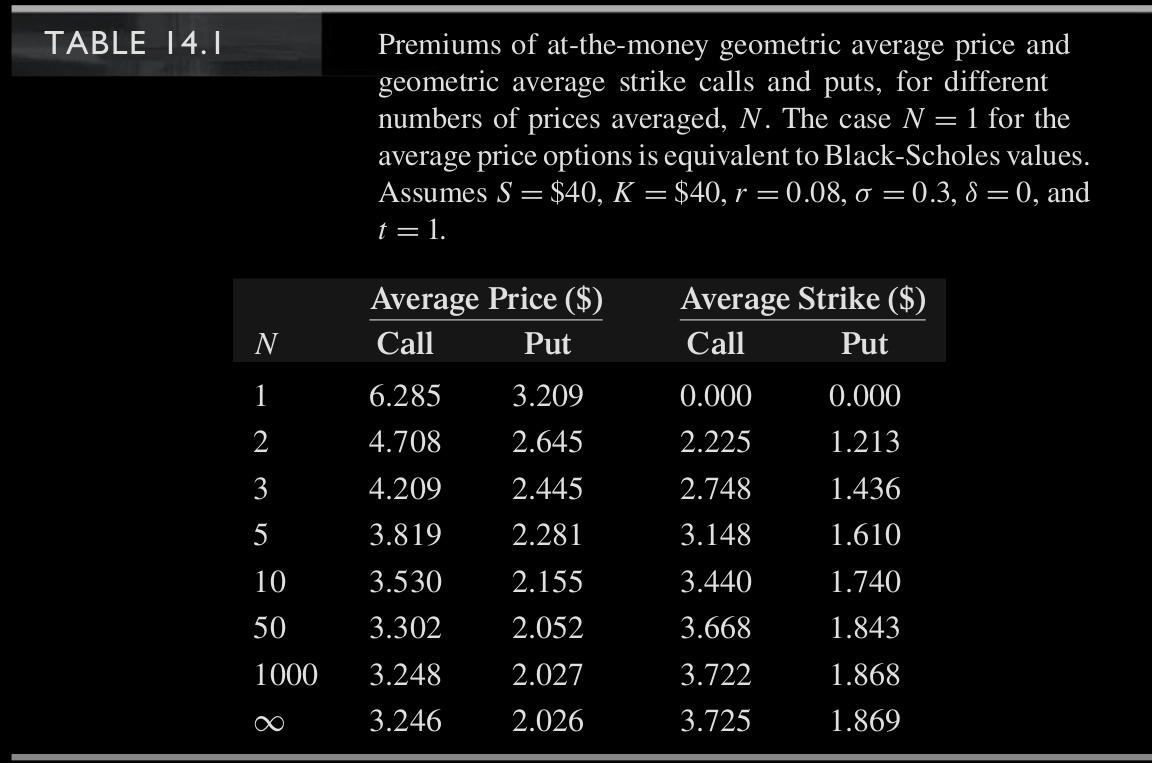
\includegraphics[scale=0.22]{figs/Table14-1.png}
	\end{center}
	\begin{mysol}
		Bonus problem... \myEnd
	\end{mysol}
\end{frame}
%-------------- end slide -------------------------------%}}}
